% Capítulo 2
\chapter{Fundamentação Teórica} \label{ch:fundamentacao-teorica}

Este capítulo apresenta uma visão geral das bases teóricas que fundamentam as
proposições  e  discussões  contidas  nesta  dissertação,  tais  como  Plataforma
Android (Seção \ref{sec:plataforma-android}), com ênfase no suporte a múltiplas
versões da API; Padrões de Projeto (Seção  \ref{sec:padroes-de-projeto}),
destacando os que foram identificados nesta pesquisa;  um Framework para Comparação
de Técnicas de Implementação de Variabilidades (Seção \ref{sec:framework}); e,
por fim, uma Taxonomia dos Componentes da API Android (Seção \ref{sec:taxonomia}). 

\section{Plataforma Android} \label{sec:plataforma-android}

Android é um sistema operacional projetado para dispositivos móveis, incluindo
celulares, tablets, relógios inteligentes, televisões e até carros. O sistema
operacional é baseado no kernel Linux, interagindo com o hardware em baixo nível
e fornecendo conjuntos de API para acesso a serviços e demais funções[REF],
apresentando uma arquitetura em camadas, conforme 

figura A. 

É sobre essa API que
os desenvolvedores irão criar suas aplicações, portanto, mudanças nela afetarão
diretamente as aplicações.

[REF]
\begin{figure}[htb]
	\centering
  	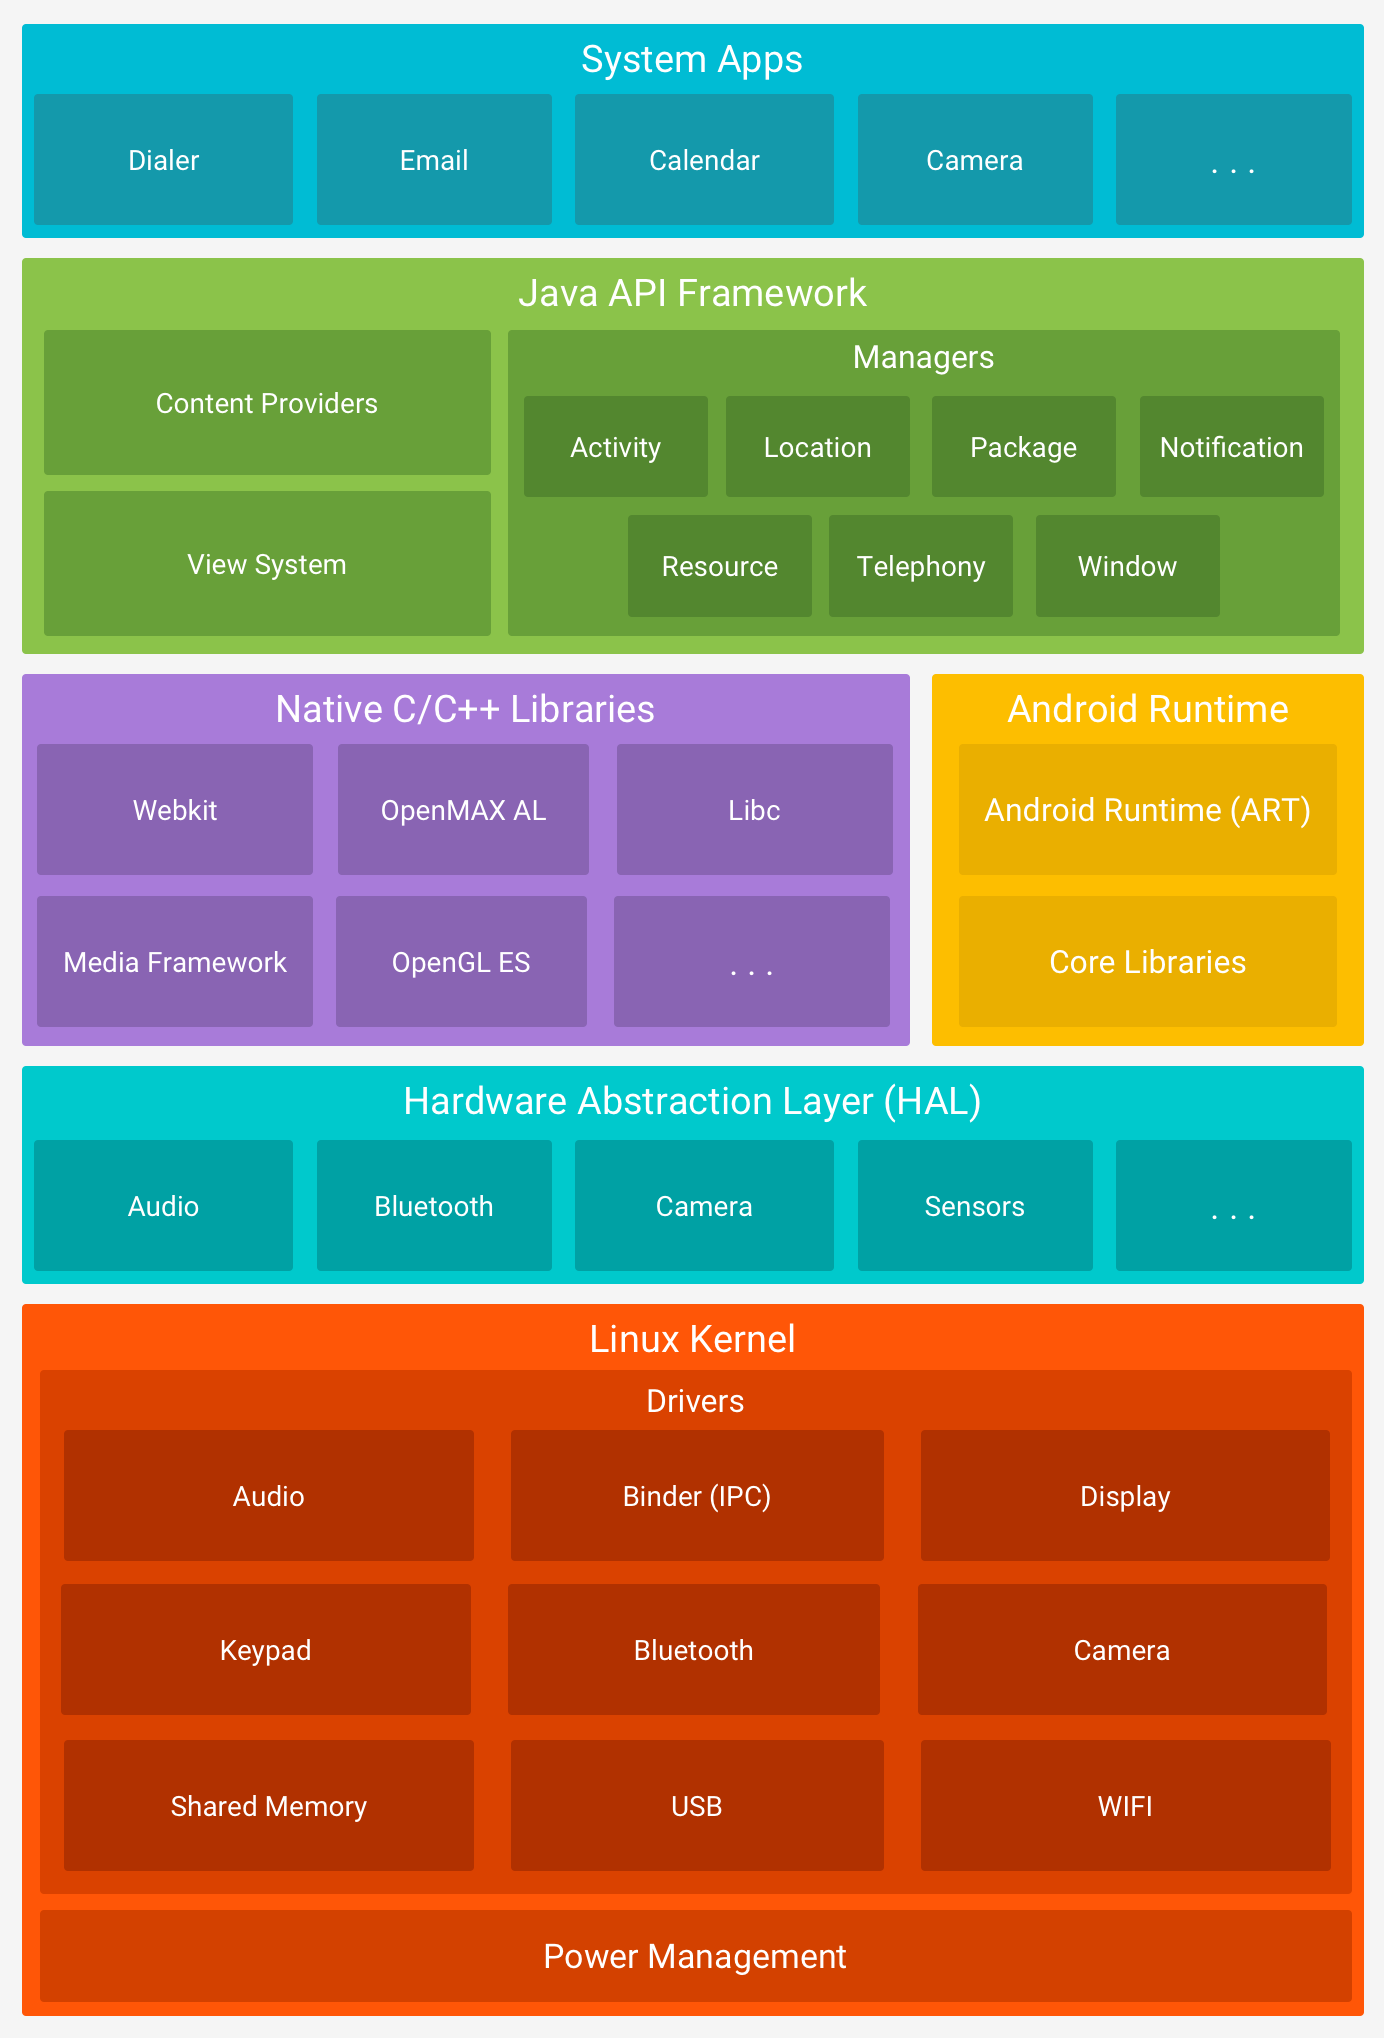
\includegraphics[scale=0.75]{imagens/android-stack_2x.png}
  	\textsf{\caption[Arquitetura em Camadas da Plataforma Android.]{Fonte: EvoSpaces \cite{Alam2007}.\label{fig:android_camadas}}}
\end{figure}

Aplicações Android são desenvolvidas em cima da camada API Java, utilizando essa
linguagem de programação, e são executadas em uma máquina virtual chamada
\abrv[DVM -- \textit{Dalvik Virtual Machine}]
{DVM}(\textit{Dalvik Virtual Machine}).
Essa máquina virtual é uma tecnologia \textit{open-source} e diferencia-se da
\abrv[JVM -- \textit{Java Virtual Machine}]
{JVM}(\textit{Java Virtual Machine}), que é baseada em pilhas, por possuir uma
arquitetura baseada em registros. Essa arquitetura permite a DVM ser executada
com pouca memória, além de possuir seu próprio \textit{bytecode}.  

\subsection{Loja de Aplicativos} \label{subsec:loja-aplicativos}

Usuários podem instalar novos aplicativos diretamente a partir de arquivos 
\abrv[APK -- \textit{Android Package}]
{APK}(\textit{Android Package}) ou obtê-los de lojas de aplicativos. A principal
lojas delas é a Google Play\footnote{https://play.google.com}, mas outras também
estão disponíveis, como Amazon Appstore\footnote{https://www.amazon.com/b/ref=nav\_shopall\_adr\_banjo?ie=UTF8\&node=11350978011}.
Na Google Play, estão disponíveis mais de 2,2 milhões de aplicativos[REF].

\subsection{Desenvolvimento de Aplicativos} \label{subsec:desenvolvimento-aplicativos}

Para criar uma aplicação Android são utilizados, 
\abrv[SDK -- \textit{Android Software Development}]
{SDK}(\textit{Android Software Development})
a linguagem de programação Java e a linguagem de marcação
\abrv[XML -- \textit{Extensible Markup Language}]
{XML}(\textit{Extensible Markup Language}). O ambiente de desenvolvimento oficial
é o Android Studio[REF], que oferece de forma integrada diversas ferramentas para
a criação de aplicações e recursos como edição de código, depuração, sistema flexível
de compilação, emuladores, ferramentas de desempenho e análise de código, como o
Android Lint[REF], que foi utilizado neste trabalho e será mais detalhado na Seção \label{subsec:android-lint}.

Uma aplicação Android consiste dos seguintes elementos:
\begin{itemize}
    \item Atividade: uma atividade é a classe onde a inferface com o usuário é
    implementada. Atividades também podem ser consideradas as tarefas que um usuários
    pode fazer em uma tela. Por exemplo, enviar um email pode ser feito em um atividade,
    enquanto escrever o email pode ser feito em outra atividade. Cada aplicação
    tem uma atividade especial chamada “atividade principal”, que é o ponto de
    entrada da aplicação[REF]. Uma aplicação contém múltiplas atividades que
    podem iniciar umas às outras para diferentes ações. Quando uma atividade
    inicia ela é colocada no topo de uma pilha chamada pilha de retorno. Quando
    o usuário pressiona o botão de voltar, a atividade atual é removida da pilha
    e a atividade anterior é exibida para o usuário. Normalmente, atividade
    removidas da pilha são destruídas e coletadas pelo coletor de lixo.
    Gerenciamento do ciclo de vida de uma aplicação é uma importante tarefa do
    desenvolvimento. Uma instância de uma atividade tem seu estado alterado entre
    diferentes possibilidades, que são:
    \begin{itemize}
        \item Ativa: atividade está na frente da tela;
        \item Pausada: atividade perdeu o foco, mas ainda é visível;
        \item Parada: atividade está completamente oculta por outra atividade;
        \item Destruída: quando parada ou pausada, o sistema encerra da atividade.
    \end{itemize}
    Para cada estado, o sistema chama uma série de métodos do ciclo de vida[REF],
    apresentada na 
    
    figura C.  
    
    O método “onCreate” é chamada quando a atividade é
    iniciada pela primeira vez, método “onStart” é chamado quando a atividade
    torna-se visível para o usuário, “onRestart” é chamado quando a atividade
    pausada mas não destruída é novamente iniciada, “onResume” é  chamado quando
    a atividade inicia a interação com o usuário, “onPause” é chamado quando o
    sistema inicia a atividade anterior, “onStop” é chamado quando a atividade
    não é mais visível, “onDestroy” é o método final chamado antes da atividade
    ser destruída pelo sistema[REF]. 
    
    [REF]
    \begin{figure}[htb]
    	\centering
      	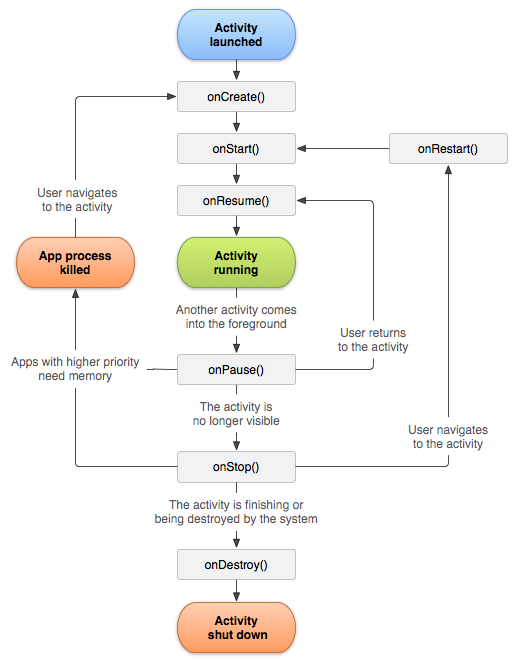
\includegraphics[scale=0.75]{imagens/activity_lifecycle.png}
      	\textsf{\caption[Ciclo de vida da atividade.]{Fonte: EvoSpaces \cite{Alam2007}.\label{fig:android_camadas}}}
    \end{figure}


    \item Contexto: contexto é responsável por capturar informações sobre o ambiente.
    Esses componentes contêm o estado atual da atividade ou aplicação e informações
    globais sobre a aplicação. Eles permitem acessar recursos específicos da aplicação,
    classes e operações em nível de aplicação como executar atividades [REF].
    \item Serviço: um serviço é um componente da aplicação que persiste por um
    longo tempo em \textit{background}, o que significa dizer que não tem uma
    interface com o usuário. Uma das mais importantes propriedade dos serviços é
    que eles podem executar em \textit{background} mesmo que o usuário alterne entre aplicações [REF]. 
    \item Intenção: intenção é o objeto usado para comunicação entre componentes
    de uma aplicação. Existem três importantes usos de intenções: iniciar uma
    atividade, iniciar um serviço e entregar um \textit{broadcast} [REF].
    \item Provedor de conteúdo: provedores de conteúdo podem ser considerados
    como gerenciadores de acesso a servidores de dados para um conjunto estruturado
    de dados. Eles são a padronização para transmissão de dados entre processos [REF].
    \item Receptor de mensagem: um receptor de mensagem é usado para executar uma
    aplicação para responder a eventos enviados para todos o dispositivos, tais
    como o recebimento de uma mensagem de texto ou notificação de baixa carga de bateria [REF].
\end{itemize}



\section{Suporte a múltiplas versões da API} \label{sec:suporte-multiversao}

Um aspecto chave no desenvolvimento de aplicações Android são as versões da API.
Google disponibilizou a primeira versão do Android (Android 1.0, API 1) em setembro
de 2008, desde então uma nova versão da API é disponibilizada aproximadamente a
cada 3 meses. Nesse momento, a última versão disponibilizada é a 24. Para este
trabalho foram consideradas, por questões de padronização das análises, configuração
do ambiente de desenvolvimento e mercado, aplicações que usaram até a versão 23.

Apesar da rápida evolução do Android, a adoção das novas API’s é lenta e o mercado
consumidor é fragmentado em relação ao número de versões da API. O que obriga os
desenvolvedores de aplicações a tomarem decisões de projeto como usar as versões
mais recentes da API e deixar de lado um mercado consumidor que não usa determinada
API ou atender a esse mercado consumidor mas não usar as novidades da API mais recente.

Para auxiliar nessa decisão, o Google disponibiliza estatísticas de uso das versões da
API[REF], conforme mostra a 

figura V, 

e mecanismos para o suporte a múltiplas versões.
Ou seja, é possível atender um usuário com baixa versão de API ao mesmo tempo que
é possível usar recursos mais modernos da plataforma. Tais mecanismos são apresentadas
nas seções seguintes.

[REF]
\begin{figure}[htb]
	\centering
  	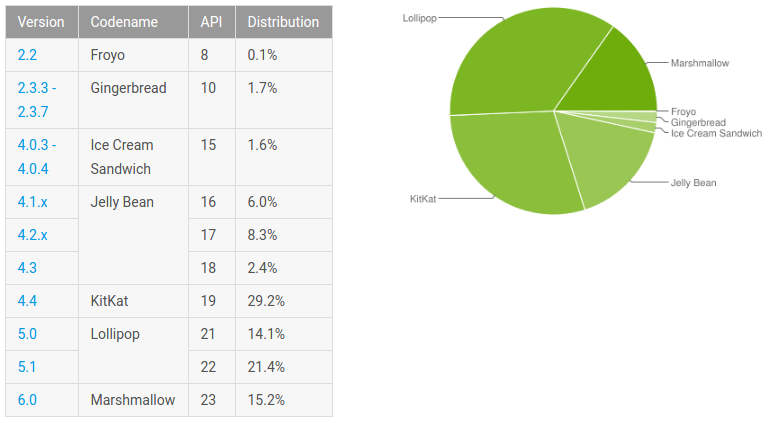
\includegraphics[scale=0.75]{imagens/platform_versions.png}
  	\textsf{\caption[Distribuição da versão da API do Android.]{Fonte: EvoSpaces \cite{Alam2007}.\label{fig:android_camadas}}}
\end{figure}

Embora 23 versões da API tenha sido lançadas, na 

figura V 

são apresentadas somente 10 versões. Isso ocorre porque versões com uma
distribuição inferior a 0,1\% são omitidas. 


\subsection{Pacote de Compatibilidade} \label{subsec:pacote-compatibilidade}

Pacotes de compatibilidade [REF], ou bibliotecas de suporte,  permitem que aplicações
em execução sob versões antigas da plataforma utilizem recursos que foram
disponibilizadas em versões mais novas. Por exemplo, uma aplicação instalada em
um aparelho com API de nível 8 pode usar a API de fragmentos, disponibilizada
apenas no nível 11.

Esses pacotes são tradicionais arquivos JAR com classes, interfaces e outros
artefatos de recursos que poderão ser adicionados na aplicação. Assim, quando se
deseja usar a classe \texttt{Fragment}, por exemplo, em vez da importação ser da API
padrão do Android, como mostra a 

Figura 3, 

deverá ser feita desse pacote que
está junto da aplicação, como mostrado na 

Figura 4.

\begin{figure}[htb]
	\centering
  	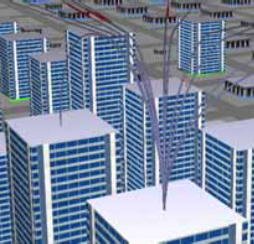
\includegraphics[scale=0.75]{Imagens/evospaces.png}
  	\textsf{\caption[EvoSpaces.]{EvoSpaces \cite{Alam2007}.\label{fig:evospaces}}}
\end{figure}


\begin{figure}[htb]
	\centering
  	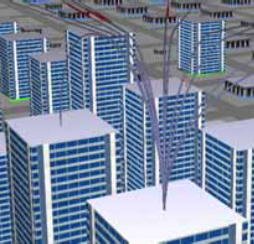
\includegraphics[scale=0.75]{Imagens/evospaces.png}
  	\textsf{\caption[EvoSpaces.]{EvoSpaces \cite{Alam2007}.\label{fig:evospaces}}}
\end{figure}

Como resultado, a aplicação será distribuída com uma experiência de uso mais consistente
através de um grande número de versões da plataforma.

\subsection{Re-implementação de recursos} \label{subsec:reimplementacao-recursos}

Re-implementação de recursos ocorre quando se deseja um comportamento já provido
por versões mais recentes ou outra biblioteca, mas opta-se por re-implementar tal
recurso. Tal implementação pode ocorrer de três formas:

\begin{itemize}
    \item Re-implementação própria;
    \item Cópia do código-fonte da API padrão[REF] [REF];
    \item Cópia do código-fonte de biblioteca de terceiro que implementa o recurso [REF].
\end{itemize}

Foi verificado que 14 de 25 aplicações analisadas optaram por essa abordagem. Entre
elas, o aplicativo de mensagens Telegram ao re-implementar algumas classes relacionadas a animações gráficas, quando poderia ter utilizado um pacote de compatibilidade com o recurso pronto. A 

figura 7 

apresenta a estrutura de pacotes do Telegram, com destaque para as classes que
re-implementam o pacote \texttt{android.animation} da plataforma, provento
funcionalidades de animação para a aplicação, mesmo em dispositivos com nível da
API inferior a 11, quando esse pacote foi disponibilizado.

\begin{figure}[htb]
	\centering
  	\frame{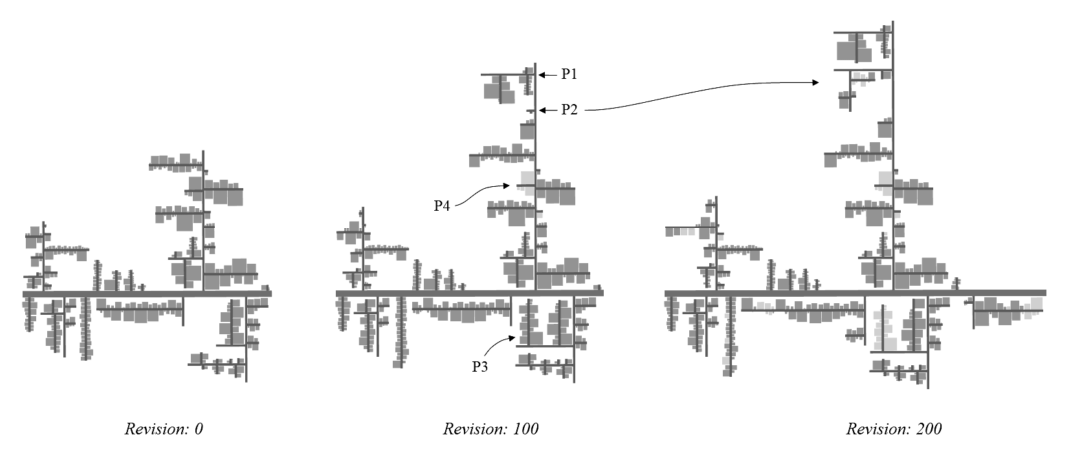
\includegraphics[scale=0.40]{Imagens/crococosmos.png}}
  	\textsf{\caption[CrocoCosmos.]{CrocoCosmos \cite{Steinbruckner2010b}.\label{fig:crococosmos}}}
\end{figure}

\subsection{Uso explícito da nova API} \label{subsec:uso-explicito-nova-api}

Uso explícito da nova API ocorre quando é feita uma chamada a um novo recurso da
API, disponibilizado apenas em uma versão da API superior a mínima exigida para
execução da aplicação [REF]. A 

figura N 

apresenta um alerta do Android Studio indicando uma chamada para um método da API
nível 11, em uma aplicação que poderá ser instalada em qualquer aparelho com API
igual ou superior a nível 4.

\begin{figure}[htb]
	\centering
  	\frame{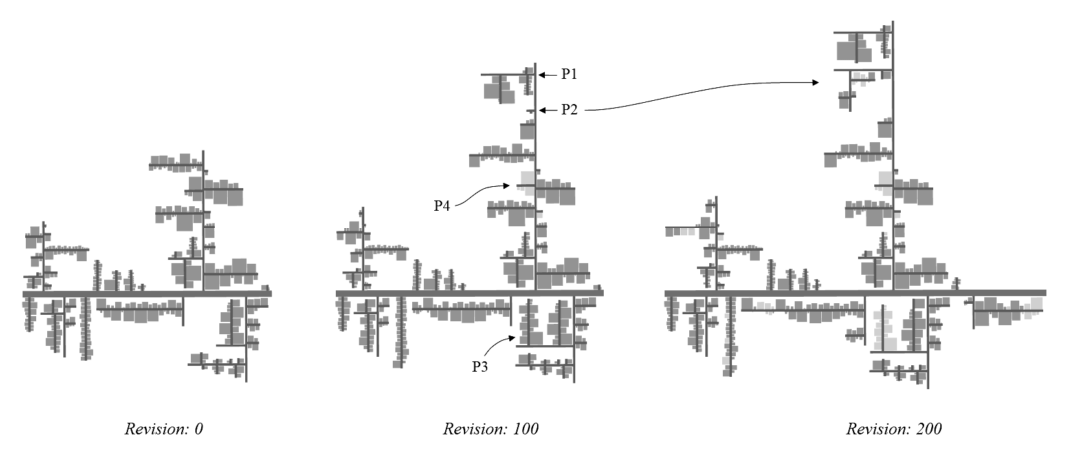
\includegraphics[scale=0.40]{Imagens/crococosmos.png}}
  	\textsf{\caption[CrocoCosmos.]{CrocoCosmos \cite{Steinbruckner2010b}.\label{fig:crococosmos}}}
\end{figure}


Caso a chamada seja realmente feita durante a execução da aplicação, será lançada
uma exceção e a aplicação será interrompida, causado uma má experiência de uso.
Dessa forma, é necessário proteger tal chamada, fazendo com que ela só seja realmente
executada em ambientes seguros, no caso, em versões da API igual ou superior a 11.
As seções seguintes apresentam soluções de projeto que podem ser utilizadas para
proteger usos explícitos de novas API’s. 

\section{Execução condicional } \label{sec:execucao-condicional}

Execução condicional (EC) é um padrão para tratar variabilidades em granularidade
fina em linhas de produto de software [REF]. O padrão é composto por 4 elementos
principais, ilustrados na 

Figura 5:

\begin{itemize}
    \item Classes alvo: componentes do sistema onde ocorre a variabilidade acontece; 
    \item Implementação da variabilidade: o código que representa a variabilidade,
    podendo ser um trecho diretamente na classe algo ou uma chamada para um componente
    que implementa a variabilidade; 
    \item Gerenciador da execução: é um elemento central do padrão, responsável
    por decidir qual implementação da variabilidade será executada;
    \item Repositório de parâmetros:  responsável por armazenar os valores dos
    parâmetros que será utilizado durante a execução condicional. É fundamental
    que a recuperação desses parâmetros não prejudique o desempenho das aplicações.
\end{itemize}


\begin{figure}[htb]
	\centering
  	\frame{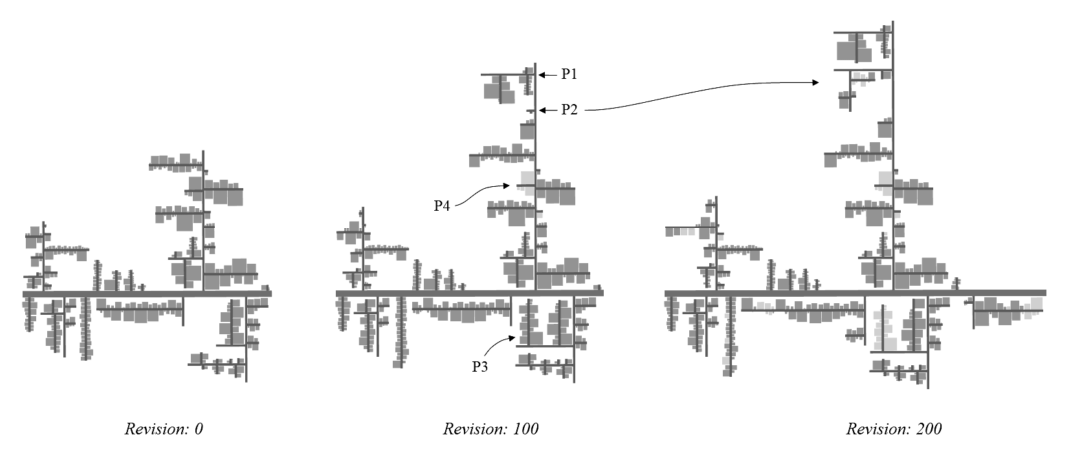
\includegraphics[scale=0.40]{Imagens/crococosmos.png}}
  	\textsf{\caption[CrocoCosmos.]{CrocoCosmos \cite{Steinbruckner2010b}.\label{fig:crococosmos}}}
\end{figure}

Em aplicações Android, as classes alvo podem ser qualquer classe da aplicação.
Gerenciador de execução é uma instrução \texttt{if} que compara a versão da API
no dispositivo e uma versão cujo valor tem alguma importância para a variabilidade
em questão. Por exemplo, a versão em que um recurso surgiu ou mudou de comportamento.
Implementação da variabilidade costuma ser uma sequência de código para quando o
resultado dessa comparação é verdadeiro e outra sequência para quando ele é falso.
O repositório de parâmetros que armazenar os valores utilizados nesse contexto é
a classe \texttt{android.os.Build}, que contém diversas informações sobre o
sistema instalado no aparelho, e suas classes aninhadas \texttt{VERSION} e \texttt{VERSION\_CODES}.
Em particular, a versão da API é obtida no atributo \texttt{Build.VERSION\_CODE.SDK\_INT},
já o outro valor da comparação é normalmente definida diretamente no código ou obtido de \texttt{VERSION\_CODES}.

A 

figura 3.2.1.1.2b 

apresenta um exemplo do uso de EC na aplicação C:geo. A classe \texttt{AbstractDialogFragment}
 é a classe alvo no padrão, do repositório de parâmetros são obtidos os valores
 de \texttt{Build.VERSION.SDK\_INT} e \texttt{Build.VERSION\_CODES.HONEYCOMB},
 que serão utilizados na condição do \texttt{if...else},  que faz o papel de gerenciador
 de execução. Também vemos que existem duas implementação de variabilidade:
 i) uma composta apenas por uma linha de código ( \texttt{view.showContextMenu()}); e 
 ii) a outra composta por várias linhas e encapsulada no método \texttt{showPopupHoneycomb(View view)}.
 
\begin{figure}[htb]
	\centering
  	\frame{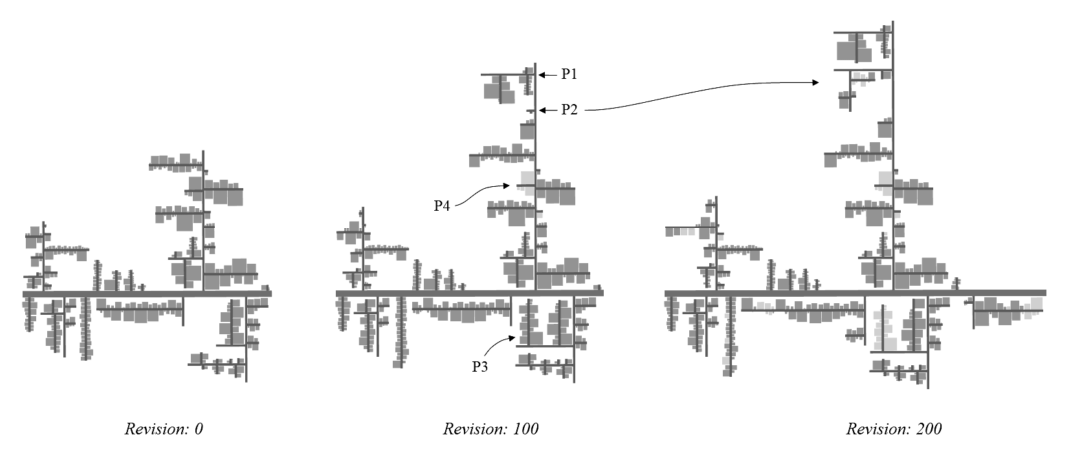
\includegraphics[scale=0.40]{Imagens/crococosmos.png}}
  	\textsf{\caption[CrocoCosmos.]{CrocoCosmos \cite{Steinbruckner2010b}.\label{fig:crococosmos}}}
\end{figure}
 

Execução condicional é a forma indicada na documentação oficial[REF] para o
suporte a múltiplas versões. Podem ser utilizada em sua forma mais simples, como
no exemplo acima, ou combinado com padrões de projeto, como apresentado na seção seguinte.

Existem no mercado várias ferramentas que realizam a medição do atributo de qualidade de desempenho para a linguagem Java. Algumas delas são:
\begin{itemize}
	\item \textit{VisualVM} \cite{Vis}: distribuída gratuitamente com o \textit{Java Development Kit} (JDK), exibe o tempo de execução de cada método em tempo real e o usuário pode, à medida que deseja, tirar fotografias instantâneas da execução do software, os chamados \textit{snapshots};
	\item \textit{JProfiler} \cite{JProfiler}: ferramenta paga, pode exibir o \textit{call graph} de chamadas dos métodos em tempo real, com seus respectivos tempos de execução. Assim como o \textit{VisualVM}, a ferramenta oferece a possibilidade de guardar \textit{snapshots} de determinados momentos da execução;
	\item \textit{YoutKit Java Profiler} \cite{Profiler2016}: ferramenta paga que possui funcionalidades semelhantes às do \textit{JProfiler}.
\end{itemize}

\subsection{Android Lint} \label{sec:android-lint}

Android Lint [REF] é uma ferramenta do ambiente oficial de desenvolvimento de
aplicações Android capaz de analisar o código-fonte de uma aplicação para
identificar problemas estruturais, sem a necessidade de executá-la ou mesmo escrever testes.

Usos explícitos da nova API, portanto chamadas a elementos que não estão presentes
na versão mínima de API exigida pela aplicação, são exemplos de problemas estruturais,
podendo levar a falhas na execução, seja algum comportamento inesperado ou até
mesmo interrupção da aplicação. Existem duas centenas de verificações feitas pelo
Lint[REF]. Duas delas verificam por acesso a elementos
adicionados à API em versões superiores à versão mínima exigida pela aplicação: 
InlinedApi e NewApi.

InlinedApi verifica por acessos a constantes. Durante o build da aplicação os
valores dessas constantes serão copiados para os arquivos das classes que as
referenciam, o que significa dizer que os valores sempre estarão disponíveis,
mesmo executando em dispositivos com API antigas. Em alguns casos não haverá
problemas, em outros isso pode resultar em interrupção da execução ou comportamento
incorreto. Dependerá do contexto, então os desenvolvedores deverão avaliar com
cuidado se o código poderá ser executado em qualquer situação ou não.

NewApi verifica por chamadas a métodos e referências a classes. Como chamadas a
métodos só podem ser resolvidas em tempo de execução, será lançada uma exceção do
tipo \texttt{java.lang.NoSuchMethodError}, ou similar, levando ao travamento da
aplicação, sempre que a chamada for feita em dispositivos com API antigas.

Dessa forma, nessa dissertação de mestrado focaremos apenas nas ocorrências de NewApi.


\section{Framework para Comparação de Técnicas de Implementação de Variabilidades} \label{sec:framework}

As diversas versões de API existentes na plataforma Android, em um contexto de
engenharia de linha de produtos de software (LPS) [REF],
são conhecidas como variabilidades. Existem diversas técnicas para implementação
de variabilidades, de forma que se faz necessários critérios de comparação e
seleção de qual utilizar em uma determinada situação. propôs um framework para
comparação de tais técnicas. O framework é uma extensão de outros trabalhos [REF] [REF],
cujos critérios de avaliação e valores possíveis estão apresentados na 

Tabela F.

\begin{table}[h]
  \caption{Framework para comparação de técnicas de implementação de variabilidades}
  \begin{tabular}{ | l | l |}
    \hline
    \textbf{Critério de avaliação} & \textbf{Valores possíveis}  \\ \hline
    Tipo de variabilidade & Positivo, negativo ou ambos  \\ \hline
    Variabilidade na estrutura & Oferece suporte ou não oferece suporte \\ \hline
    Variabilidade no comportamento & Oferece suporte ou não oferece suporte \\ \hline
    Granularidade & Fina ou grossa \\ \hline
    Tempo de ligação & Pré-processamento, compilação, implantação, execução \\ \hline
    Reusabilidade & Alta, média, ou baixa \\ \hline
    Legibilidade & Alta, média, ou baixa \\ \hline
    Desempenho & Alta, média, ou baixa \\ \hline
    Tamanho da aplicação & Alto impacto ou baixo impacto \\ \hline
    \begin{tabular}[c]{@{}l@{}}Suporte para implementação\\ modular de requisitos transversais\end{tabular}  & Oferece suporte ou não oferece suporte \\ \hline
  \end{tabular}
  \label{tab:framework}
\end{table}

\textbf{Tipo de variabilidade} indica a adição ou remoção de comportamento ou
estrutura quando comparada com uma implementação base. \textbf{Variabilidade na estrutura}
indica a possibilidade de estaticamente organizar elementos do programa,
como adição de métodos ou atributos em classes, enquanto \textbf{variabilidade no comportamento}
diz respeito a diferentes semânticas de execução. \textbf{Granularidade fina}
refere-se avariações em nível de métodos de classe, incluindo trechos no corpo
dos métodos, ao passo que \textbf{granularidade grossa} é uma variação em nível
de classes. \textbf{Tempo de ligação} indica o momento durante o desenvolvimento
em que as decisões acerca da variação tem que ser tomada, por exemplo,
uma variação pode ser tratada durante a compilação ou somente no momento da execução.

Outros parâmetros importantes para avaliação são \textbf{reusabilidade}, \textbf{legibilidade},
\textbf{tamanho da aplicação} e \textbf{desempenho}, esses dois últimos dizem
respeito a um produto executável da LPS.

Também é considerado o suporte para implementação modular de requisitos transversais.
Esse suporte é importante porque muitas variabilidades de LPS podem ser requisitos
transversais, como apontado por diversas pesquisas [REF] [REF] [REF] [REF] [REF].

\section{Padrões de Projeto} \label{sec:padroe-projeto}

\section{Taxonomia dos Componentes da API} \label{sec:taxonomia}



